% Free Body Diagram
% Demonstrates: force vectors, decomposition, angles, and labels for mechanics.
% Compile with: pdflatex main.tex

\documentclass[border=10pt]{standalone}
\usepackage{tikz}
\usetikzlibrary{angles, quotes, calc, arrows.meta, decorations.pathmorphing}

\begin{document}
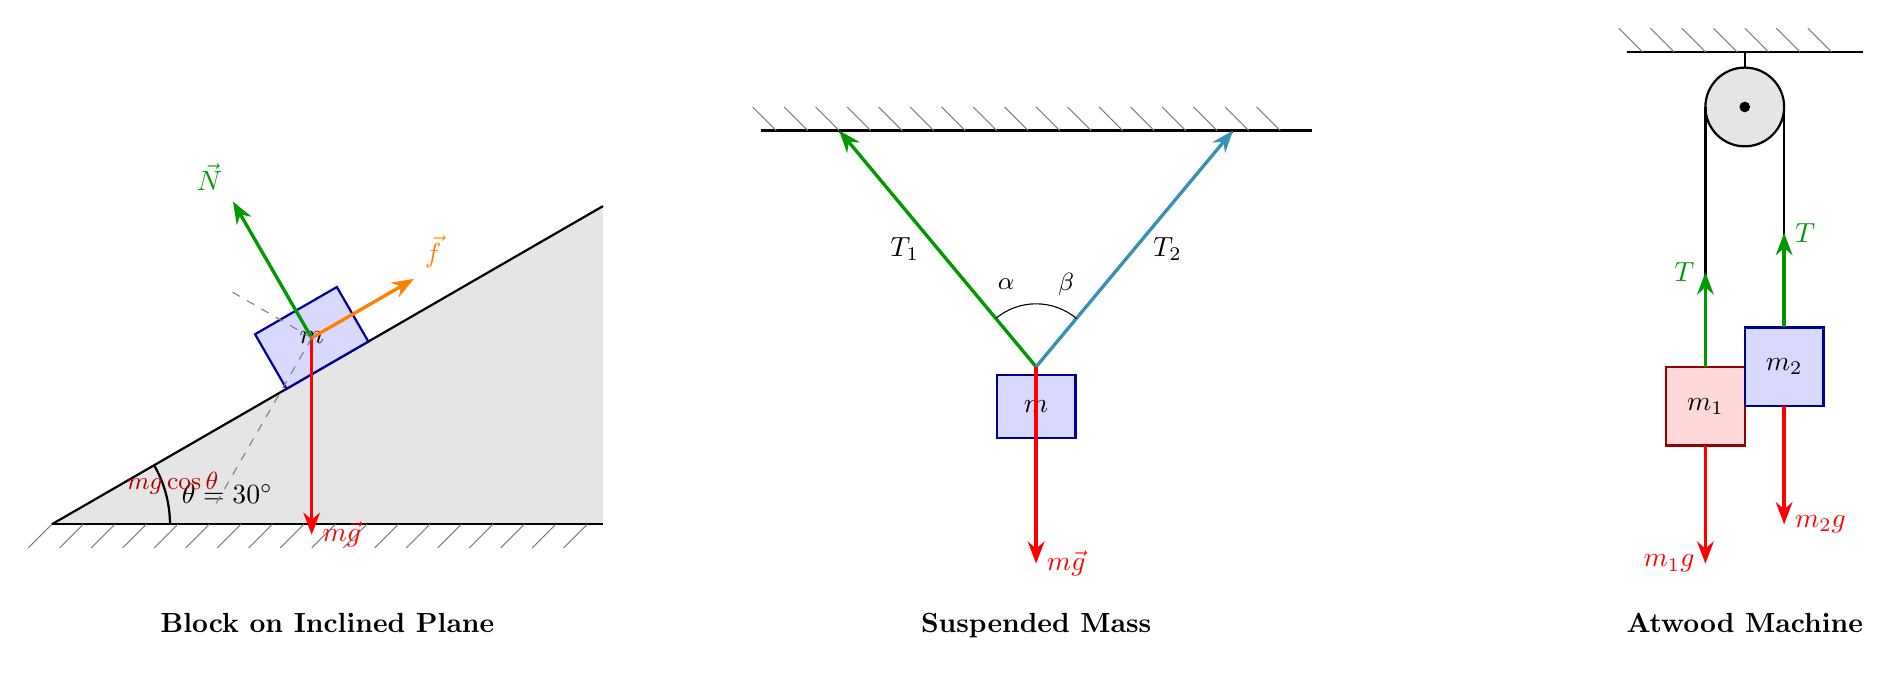
\begin{tikzpicture}[
    >=Stealth,
    force/.style={very thick, -{Stealth[length=8pt]}},
    dashed line/.style={dashed, gray, thin},
]

% =============================================================================
% Scene 1: Block on an inclined plane
% =============================================================================
\begin{scope}[shift={(0,0)}]

    % --- Inclined plane ---
    \def\ang{30}
    \def\blockw{1.2}
    \def\blockh{0.8}

    % Ground and slope
    \fill[gray!20] (0,0) -- (7,0) -- (7,{7*tan(\ang)}) -- cycle;
    \draw[thick] (0,0) -- (7,0);
    \draw[thick] (0,0) -- (7,{7*tan(\ang)});

    % Angle arc
    \draw[thick] (1.5,0) arc[start angle=0, end angle=\ang, radius=1.5]
        node[midway, right=2pt] {$\theta = \ang^\circ$};

    % Hatching on ground
    \foreach \x in {0,0.4,...,7} {
        \draw[gray, thin] (\x, 0) -- ++(-.3, -.3);
    }

    % --- Block (rotated to sit on slope) ---
    \coordinate (center) at (3.5, {3.5*tan(\ang)+0.55});

    \begin{scope}[rotate around={\ang:(3.5,{3.5*tan(\ang)})}]
        \coordinate (block) at (3.5, {3.5*tan(\ang)});
        \filldraw[fill=blue!15, draw=blue!60!black, thick]
            ([shift={(-\blockw/2,0)}]block) rectangle
            ([shift={(\blockw/2,\blockh)}]block);
        \node at ([shift={(0,\blockh/2)}]block) {$m$};
        \coordinate (C) at ([shift={(0,\blockh/2)}]block);
    \end{scope}

    % --- Forces from center of block ---
    % Weight (straight down)
    \draw[force, red] (C) -- ++(0, -2.5)
        node[right, pos=1] {$m\vec{g}$};

    % Normal force (perpendicular to slope)
    \draw[force, green!60!black] (C) -- ++({-2*sin(\ang)}, {2*cos(\ang)})
        node[above left, pos=1] {$\vec{N}$};

    % Friction (up the slope)
    \draw[force, orange] (C) -- ++({1.5*cos(\ang)}, {1.5*sin(\ang)})
        node[above right, pos=1] {$\vec{f}$};

    % Weight components (dashed)
    \draw[dashed line] (C) -- ++({-2.5*sin(\ang)}, {-2.5*cos(\ang)})
        node[left, pos=0.85, font=\small, text=red!70!black] {$mg\cos\theta$};
    \draw[dashed line] (C) -- ++({-1.2*cos(\ang)}, {1.2*sin(\ang)});

    \node[font=\bfseries, anchor=north] at (3.5, -1) {Block on Inclined Plane};
\end{scope}

% =============================================================================
% Scene 2: Suspended mass with two ropes
% =============================================================================
\begin{scope}[shift={(10, 0)}]

    % --- Ceiling ---
    \draw[thick] (-1, 5) -- (6, 5);
    \foreach \x in {-0.8,-0.4,...,6} {
        \draw[gray, thin] (\x, 5) -- ++(-0.3, 0.3);
    }

    % --- Attachment points ---
    \coordinate (L) at (0, 5);
    \coordinate (R) at (5, 5);
    \coordinate (M) at (2.5, 2);

    % --- Ropes ---
    \draw[thick] (L) -- (M) node[midway, left=3pt] {$T_1$};
    \draw[thick] (R) -- (M) node[midway, right=3pt] {$T_2$};

    % --- Mass ---
    \filldraw[fill=blue!15, draw=blue!60!black, thick]
        ($(M)+(-0.5,-0.1)$) rectangle ($(M)+(0.5,-0.9)$);
    \node at ($(M)+(0,-0.5)$) {$m$};

    % --- Forces at junction ---
    % Tension 1
    \draw[force, green!60!black] (M) -- ++($(L)-(M)$)
        coordinate (T1end);
    \path (M) -- (T1end) node[midway, left=5pt] {};

    % Tension 2
    \draw[force, cyan!70!black] (M) -- ++($(R)-(M)$)
        coordinate (T2end);

    % Weight
    \draw[force, red] (M) -- ++(0, -2.5) node[right, pos=1] {$m\vec{g}$};

    % --- Angles ---
    \coordinate (Mup) at ($(M)+(0,1)$);
    \pic[draw, angle radius=0.8cm, "$\alpha$" font=\small, angle eccentricity=1.4]
        {angle = Mup--M--L};
    \pic[draw, angle radius=0.8cm, "$\beta$" font=\small, angle eccentricity=1.4]
        {angle = R--M--Mup};

    \node[font=\bfseries, anchor=north] at (2.5, -1) {Suspended Mass};
\end{scope}

% =============================================================================
% Scene 3: Pulley system
% =============================================================================
\begin{scope}[shift={(19, 0)}]

    % --- Support ---
    \draw[thick] (1, 6) -- (4, 6);
    \foreach \x in {1.2,1.6,...,4} {
        \draw[gray, thin] (\x, 6) -- ++(-.3, .3);
    }

    % --- Pulley ---
    \draw[thick, fill=gray!20] (2.5, 5.3) circle (0.5);
    \filldraw[black] (2.5, 5.3) circle (0.06);
    \draw[thick] (2.5, 6) -- (2.5, 5.8);

    % --- Rope ---
    \draw[thick] (2.0, 5.3) -- (2.0, 2) node[midway, left=3pt] {};
    \draw[thick] (3.0, 5.3) -- (3.0, 2.5) node[midway, right=3pt] {};

    % --- Mass 1 (left) ---
    \filldraw[fill=red!15, draw=red!60!black, thick]
        (1.5, 1) rectangle (2.5, 2);
    \node at (2, 1.5) {$m_1$};

    % --- Mass 2 (right) ---
    \filldraw[fill=blue!15, draw=blue!60!black, thick]
        (2.5, 1.5) rectangle (3.5, 2.5);
    \node at (3, 2) {$m_2$};

    % --- Forces ---
    % m1: weight down, tension up
    \draw[force, red] (2, 1) -- ++(0, -1.5) node[left, pos=1] {$m_1 g$};
    \draw[force, green!60!black] (2, 2) -- ++(0, 1.2) node[left, pos=1] {$T$};

    % m2: weight down, tension up
    \draw[force, red] (3, 1.5) -- ++(0, -1.5) node[right, pos=1] {$m_2 g$};
    \draw[force, green!60!black] (3, 2.5) -- ++(0, 1.2) node[right, pos=1] {$T$};

    \node[font=\bfseries, anchor=north] at (2.5, -1) {Atwood Machine};
\end{scope}

\end{tikzpicture}
\end{document}
